\chapter{Termo de Abertura do projeto}

\section{EAP}
\begin{figure}[!htb]
    \center{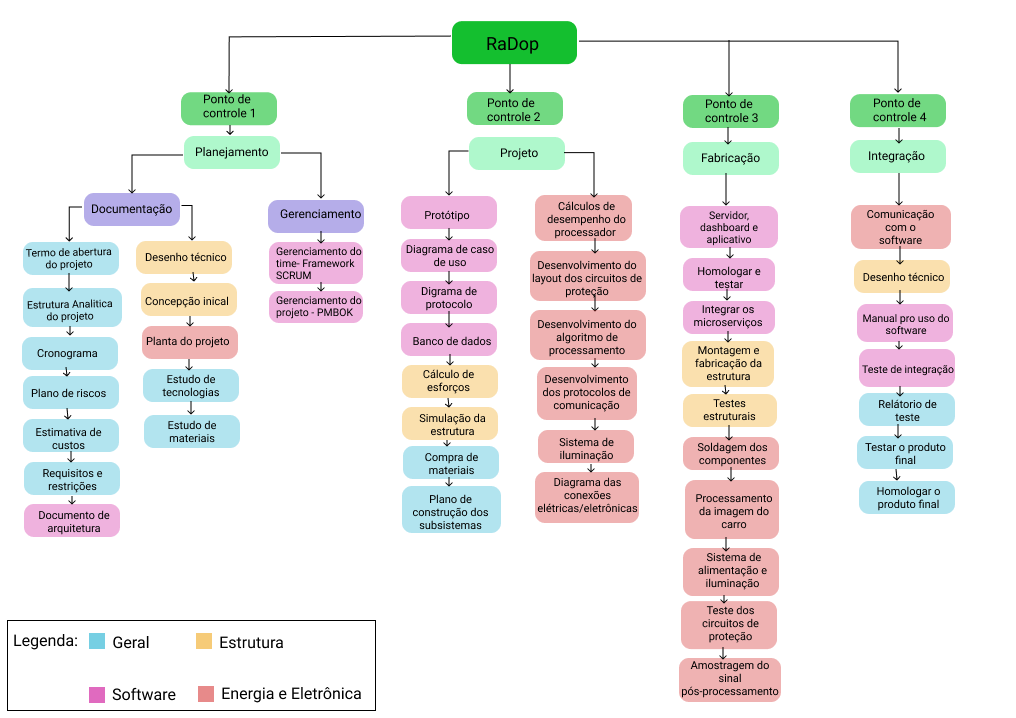
\includegraphics[width=\textwidth]{eap}}
    \caption{\label{fig:eap} EAP do projeto}
\end{figure}
\section{Lista É/Não é}
\subsection{É}
\subsection{Não é}
\section{Requisitos}
\subsection{Eletrônica}

Os requisitos de eletrônica são:
	
\begin{itemize}
	\item Detectar a aproximação do carro na via;
    \item Calcular a velocidade relativa do carro;
    \item Implementar uma comunicação entre os dois radares para determinar a emissão do alerta;
    \item Criar uma interface entre o radar e o motorista para visualização do alerta;
    \item Capturar imagem traseira do carro com a placa quando este passar acima da velocidade permitida;
    \item Projetar e construir circuitos de proteção para o dispositivos eletrônicos;
    \item Fazer o pré-processamento da imagem para reconhecimento da placa do veículo;
    \item Determinar a velocidade máxima do veículo para melhor captura da placa;
    \item Determinar a distância do veículo em relação ao radar para melhor captura da placa;
    \item Determinar a distância máxima entre os dois radares;
    \item Selecionar e implementar os protocolos de comunicação entre os dois radares;
    \item Selecionar e implementar os protocolos de comunicação entre os radares e o servidor;
     \item Determinar a capacidade de amarzenamento mínimo necessário para guardar dados quando a comunicação entre o radar e o servidor estiver fora de serviço;
     \item Determinar a velocidade mínima de transmissão de dados entre os radares para emissão de alerta;
     \item Determinar e implementar a estrutura do pacote de dados a ser enviado para o servidor contendo todas as informações necessárias;
     \item Transmitir para o servidor a velocidade, a imagem da placa pré-processada  e outras informações sobre o funcionamento do sistema.
\end{itemize}    
    
    As restrições de eletrônica são:

\begin{itemize}

	\item Se limitar em apenas reconhecer a placa do veículo, e não gerar a multa.
	\item Falha de comunicação entre os radares e o servidor por no máximo 3 dias.
	\item O veículo deve estar em uma velocidade igual ou menor que a velocidade máxima estabelecida para captura da placa.
	\item A captura da câmera deve ser apenas da traseira do veículo, devido a moto ter placa apenas na parte de trás, unificando o processo.
	\item A distância máxima entre os radares deve ser de 1 km.
	
\end{itemize} 	
	
\subsection{Energia}
\begin{itemize}
	\item O sistema deve conter painéis fotovoltaicos que promoverão a fonte de alimentação para todos os componentes do sistema;
	\item O sistema deve garantir o máximo aproveitamento energético;
	\item O sistema deve conter circuitos de controle de tensão e corrente;
	\item O sistema deve conter circuitos de controle de tensão e corrente;
	\item O sistema deve garantir o funcionamento seguro e contínuo do Radar;
	\item O sistema deve conter um circuito de iluminação para servir de alerta aos motoristas;

\end{itemize}

\subsubsection{Restrições}
\begin{itemize}
   \item Dependêcia do clima para a geração de energia;
   \item Localização Geografica;
   \item Temperatura média;
   \item Indices de radiação solar;
   \item Posicionamento das placas em relação a radiação solar;
   \item Horário de exposição;
   \item Existência de sombramento
 \end{itemize}
\subsection{Estrutura}

\subsubsection{Requisitos e restrições estruturais}

Os requisitos a serem considerados na elabora\c c\~ao e projeto estrutural dever\~ao considerar principalmente as condi\c c\~oes clim\'aticas da regi\~ao (esta\c c\~oes do ano, varia\c c\~ao de umidade e temperatura, velocidade m\'axima do vento e poss\'iveis fatores locais que possam interferir ou no funcionamento da estrutura ou no funcionamento dos componentes eletr\^onicos), al\'em das cargas geradas pelos próprios componentes estruturais. Para isso, foi realizada uma pesquisa em sites de metereologia que pudessem fornecer as informa\c c\~oes clim\'aticas da regi\~ao de Serra, onde as informações fornecidas foram retiradas do site de meteorologia do estado do Esp\'irito Santo.
A regi\~ao da Serra, de forma ampla, fica no estado do Esp\'irito Santo, na regi\~ao sudeste do Brasil, localizado na Microrregi\~ao de Vit\'oria e na Mesorregi\~ao Central Esp\'irito-Santense, como pode ser observado em \ref{mapa_es}. O clima predominante da regi\~ao sudeste litor\^anea do Brasil \'e o Tropical Atl\^antico (tropical \'umido), que apresenta grande influ\^encia da umidade vinda do Oceano Atl\^antico. As caracter\'isticas desse tipo de clima s\~ao: temperaturas elevadas no ver\~ao (podendo atingir at\'e 40$^\circ$C) e amenas no inverno (m\'edia de 20$^\circ$C), e em fun\c c\~ao da umidade trazida pelo oceano, costuma chover muito nestas \'areas.

Os dados trazidos aqui são referentes às análises estátisticas de relatórios horários adquiridos entre janeiro de 1980 e dezembro de 2016. 

\begin{figure}[h]
	\includegraphics[scale=0.2]{mapa_es}
	\centering
	\caption{Mapa regional do Estado do Espírito Santo}
	\label{mapa_es}
	
\end{figure}
Dessa forma, o clima do município de Serra é dividido da seguinte maneira:

\begin{figure}[!ht]
	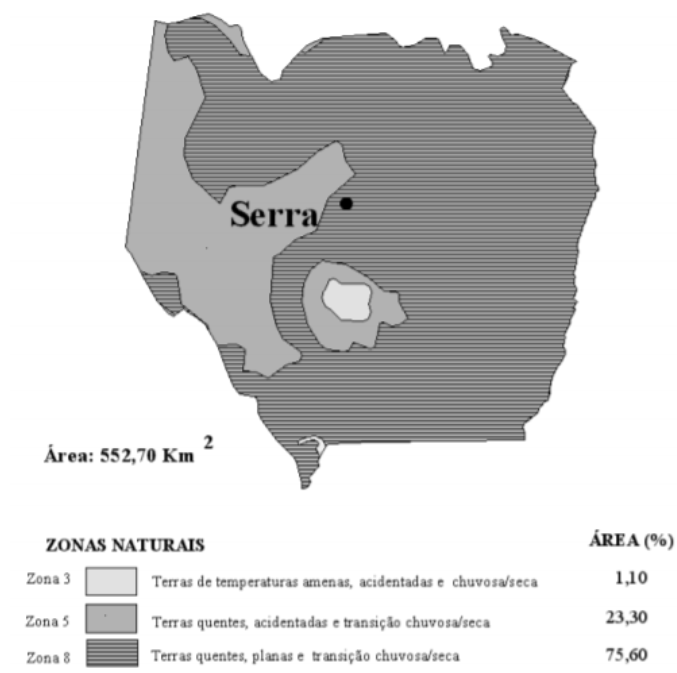
\includegraphics[scale=0.8]{reg_serra}
	\centering
	\caption{Zonas naturais da região de Serra. Fonte: Zonas Naturais do Espírito Santo (EMCAPA/NEPUT (1999))}
	\label{regiao_serra}
\end{figure}

\begin{figure}[!ht]
	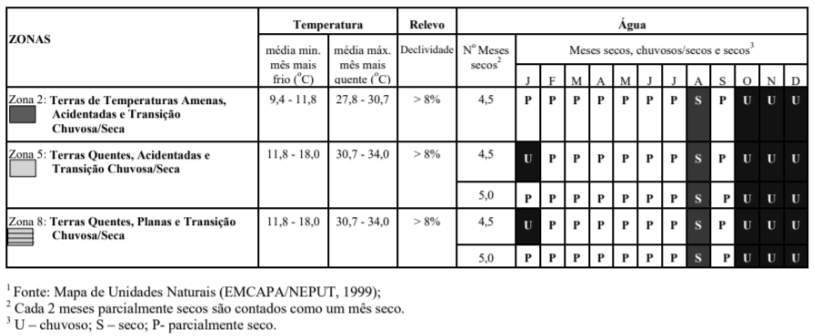
\includegraphics[scale=1]{tabela_serra}
	\centering
\end{figure}

Será considerado de forma majoritária a climatização da zona 8, por ocupar uma maior porcentagem de área na região.
Assim, foram pesquisadas de forma mais a fundo os valores médios das características climáticas da região (analisadas entre os anos de 1980 e 2016 segundo Y), tais como temperatura, nuvens, precipitação, chuva, Sol, umidade, ventos e energia solar incidente apresentados abaixo. Vale  

\subsubsection{Temperatura}

\begin{figure}[!ht]
	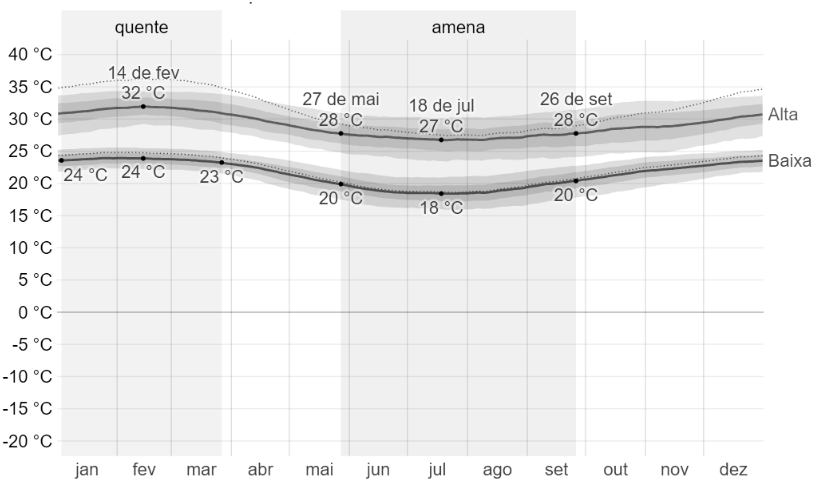
\includegraphics[scale=1]{mapa_temp}
	\centering
	\caption{Gráfico de temperatura média na região de Serra - ES.}
\end{figure}

Para o gráfico de temperaturas, é possível observar que durante o verão, a temperatura média mais alta é de 32º, enquanto durante o inverno, a mínima média é de 18º. 

\begin{figure}[!ht]
	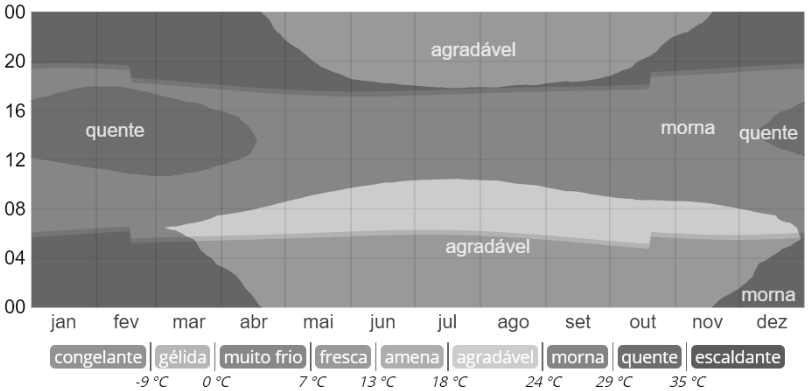
\includegraphics[scale=1]{mapa_temp2}
	\centering
	\caption{Gráfico de temperatura média horária na região de Serra - ES.}
\end{figure}

A análise gráfica dos daods de precipitação, chuva mensal e umidade severão ser analisados juntos para uma melhor interpretação pois eles se complementam.

\subsubsection{Precipitação}

\begin{figure}[!ht]
	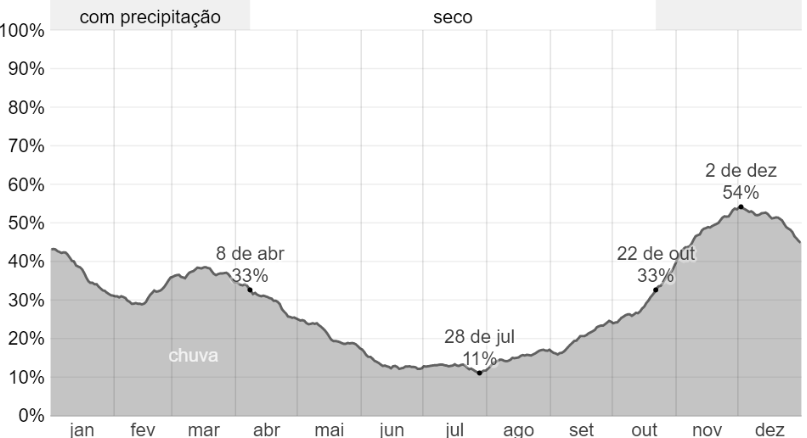
\includegraphics[scale=1]{mapa_prep}
	\centering
	\caption{Gráfico de precipitação média na região de Serra - ES.}
	\label{mapa_prep}
\end{figure}

\subsubsection{Chuva}
\begin{figure}[!ht]
	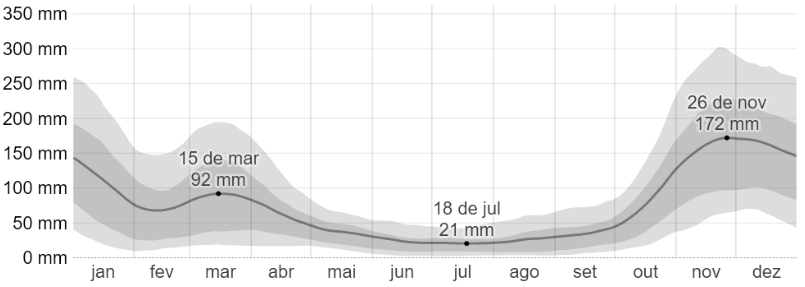
\includegraphics[scale=1]{mapa_chuva}
	\centering
	\caption{Gráfico das chuvas médias na região de Serra - ES.}
	\label{mapa_chuva}
\end{figure}
\subsubsection{Umidade}
\begin{figure}[!ht]
	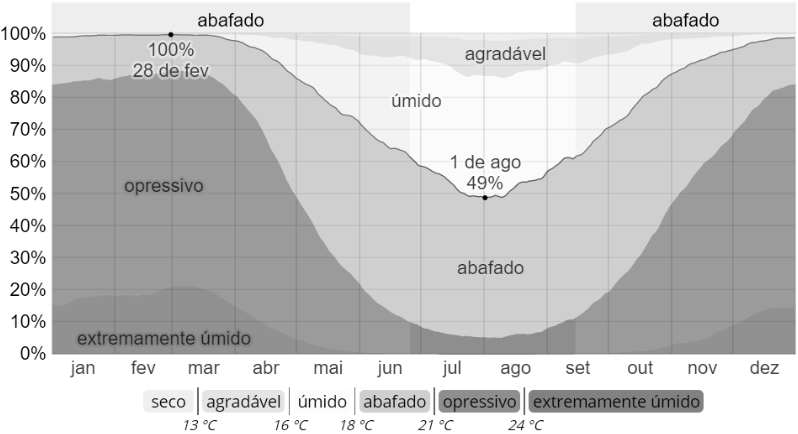
\includegraphics[scale=1]{mapa_umidade}
	\centering
	\caption{Gráfico da umidade média na região de Serra - ES.}
	\label{mapa_umidade}
\end{figure}

Análisando os gráficos \ref{mapa_prep}, \ref{mapa_chuva}, \ref{mapa_umidade} é possível relacioná-los em relação as épocas de seca e umidade, além de poder ser possível observar que os períodos quando ocorrem serem no inverno (baixas temperaturas) e verão (altas temperaturas), respectivamente. Essa análise é importante, pois além de ser necessário escolher um material que seja resistente tanto a condições de seca como de umidade, é necessário escolher um material que seja resistente à essas variações de temperatura mas que também seja ao contato constante com a chuva e umidade. Sabe-se que climas secos estão relacionados à uma variação de temperatura mais rápida entre as temperaturas máxima e mínima, enquanto dias úmidos estão relacionados à uma variação mais lenta.
 
\subsubsection{Velocidade do vento}

\begin{figure}[!ht]
	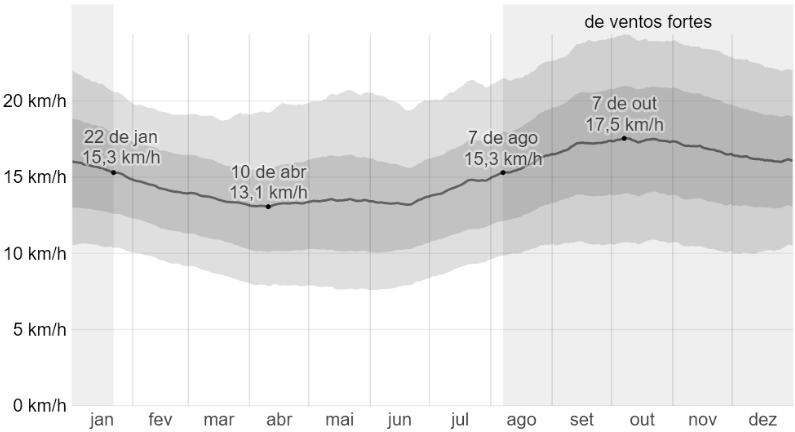
\includegraphics[scale=1]{velocidade_vento}
	\centering
	\caption{Gráfico develocidade média do vento na região de Serra - ES.}
	\label{vel_vento}
\end{figure}

Um fator mecânico importante a ser analisado é a velocidade do vento na estrutura, pois ele é responsável por esforços mecânicos que a estrutura terá que resistir. Pode-se analisar o gráfico \ref{vel_vento} e perceber que ele traz valores médios para a velocidade do mesmo. Entretanto, a fim de projetar-se uma estrutura que seja eficiente é necessário analisar a valocidade máxima do vento nos períodos de ventos fortes. Para isso, analisou-se o dia 07 de outubro que trouxe uma velocidade média acima das demais:

\begin{figure}[!ht]
	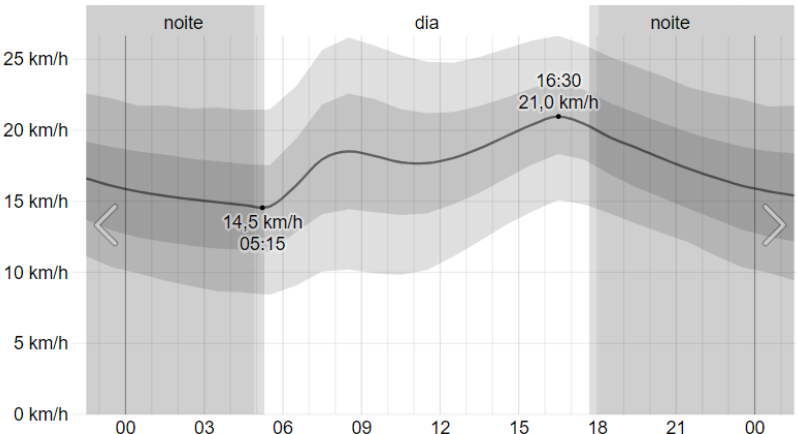
\includegraphics[scale=1]{velocidade_vento_dia07}
	\centering
	\caption{Gráfico de velocidade média do vento no dia 07 de outubro na região de Serra - ES.}
\end{figure}

Analisando as velocidades médias do vento no dia 07, vê-se que a velocidade máxima do mesmo neste dia foi de 21 Km/h. Dessa forma, é necessário perceber as variações de fatores importantes que possam interferir na eficiencia estrutural do projeto e traze-los para o projeto de forma a ter uma estrutura resistente.


\subsubsection{Incidência solar}


\begin{figure}[!ht]
	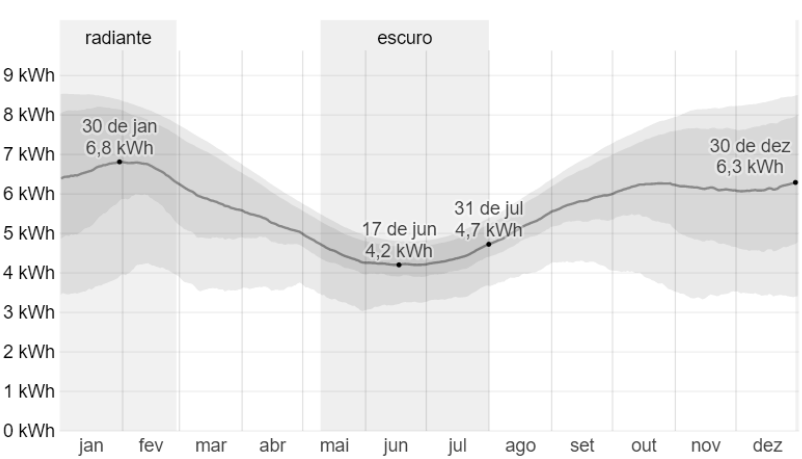
\includegraphics[scale=1]{mapa_inci_solar}
	\centering
	\caption{Gráfico da incidencia solar média nna região de Serra - ES.}
\end{figure}

É necessária uma análise da indicência solar na região levando em consideração as variações sazonais da mesma. A incidência solar é importante para o projeto em dois aspéctos: primeiro para que seja possível pesquisar materiais que sejam resistentes às ações das radiações  visíveis e também às radiações ultravioletas e, em segundo, para que seja possível fazer o projeto da placa solar que estará no topo do radar.

\subsubsection{Materiais}

O grande desafio estrutural desse projeto é conseguir aliar materiais com boas propriedades mecânicas mas que não interfiram na recepção e nem na emissão dos sinais dos componentes eletrônicos, além disso, será necessário também uma estrutura que proteja e isole os componentes eletrônicos das ações climáticas da região. 

\subsubsection{Manutenção}

É necessário projetar uma estrutura que permita o acesso de técnicos de forma segura, eficiente e rápida para manutenções periódicas (ou quando necessárias) por se tratar de um projeto que tem como áreas de atuação e instalação estradas de alta velocidade e serras.

\subsubsection{Normas}

A estrutura visa a acomodação dos componentes eletrônicos de forma segura e que
seja possível a manutenção de forma ágil, caso necessário. Além disso a estrutura
precisa possuir vazão de ar para a dissipação de calor e ao mesmo tempo
impermeável para que em caso de chuva o sistema ainda esteja protegido.

Foi levantado as dimensões mínimas para o projeto com base em documentação
disponível online no site do Conselho Nacional de Trânsito (CONATRAN).
Inicialmente foi escolhido um poste engastado com uma caixa de operação com os
componentes eletrônicos. A dimensão mínima recomendada para o poste é de 2,10
metros. A dimensões preliminares da caixa de operação são de 60cmx40cmx40cm.
Sabe-se também que a estrutura deve estar a uma distância mínima de 1,20 metros
de distância do acostamento. É necessário ser perfeitamente visível (percepção da
existência do painel), a uma distância mínima de 300m e legível (condição de leitura
e compreensão da mensagem em tempo hábil) a uma distância mínima de 270
metros. Segundo as normas do CONATRAN é necessário permitir ajustes em sua
luminosidade, em função da luminosidade ambiente e também possuir proteção anti
reflexo quando da incidência direta de luz solar.
Vale ressaltar que as dimensões aqui escolhidas para a caixa de operação e para o
poste podem sofrer alterações se for necessário a acomodação de novos
componentes ou para melhor estabilidade do sistema como um todo.

Sabe-se desde agora que o radar doppler ficará no ponto mais alto da caixa de
operações e acima da caixa ficará o painel fotovoltáico para que além do seu papel
energético ele possa servir como isolante térmico da parte superior da caixa de
operações. A disposição dos demais componentes será escolhida em conjunto com
o setor responsável pela eletrônica do projeto.

\subsubsection{Laboratórios}
Para a estrutura será utilizado o galpão da FGA e seus recursos para possíveis
processos de soldagem e reparos no projeto. A disponibilidade do mesmo já foi
pesquisada para melhor atender nossa demanda de trabalho. Eventuais processos
de fabricação serão feitos em locais próprios dos integrantes do grupo quando não
houver a necessidade ou a disponibilidade do galpão da FGA. Já foi levantado o
nome do técnico responsável para a soldagem e colaboração com a equipe de
estrutura.

\subsection{Software}

Os requisistos de software são:

\begin{itemize}
    \item Interface do Dashboard;
    \item Interface do Aplicativo;
    \item Manual de uso dos softwares (Microsserviços, Aplicativo e Dashboard);
    \item Funcionar com conexão a redes (Internet);
    \item Ser capaz de lidar e recuperar de falhas e erros (conexão, processamento e etc.);
    \item Softwares devem ser manuteníveis e evolutíveis;
    \item Softwares devem ser testáveis e testados;
    \item Software deve mostrar dados e informações do Radar;
    \item Software deve ser capaz de tomar decisões para alertar socorristas a respeito de prováveis acidentes automobilísticos;
    \item Software deve ser capaz de tomar decisões para alertar usuários de possíveis situações de risco;
    \item Software deve ser capaz de mostrar informações gerenciais com os dados do Radar;
\end{itemize}

As restrições de software são:

\begin{itemize}
    \item O software necessita estar sempre conectado à internet para comunicação e, consequentemente, para o correto funcionamento;
    \item O aplicativo de manutenção irá auxiliar apenas com o essencial;
    \item O aplicativo só funcionará em aparelhos Android;
    \item A linguagem de cada microsserviço (assim como framework/tecnologia) será definida dada necessidade (performance, armazemanento e etc) dos mesmos;
\end{itemize}

\section{\emph{Stakeholders}}
\section{Recurso humanos}

 De modo a ter uma melhor organização, a equipe foi dividida em subgrupos, onde cada subgrupo tem um gerente técnico, além disso a equipe também conta com um gerente de qualidade e um coordenador geral. Na Figura \ref{fig:organograma} mostra o organograma da equipe e o nome de cada integrante por função.
 
\begin{figure}[h]
\centering
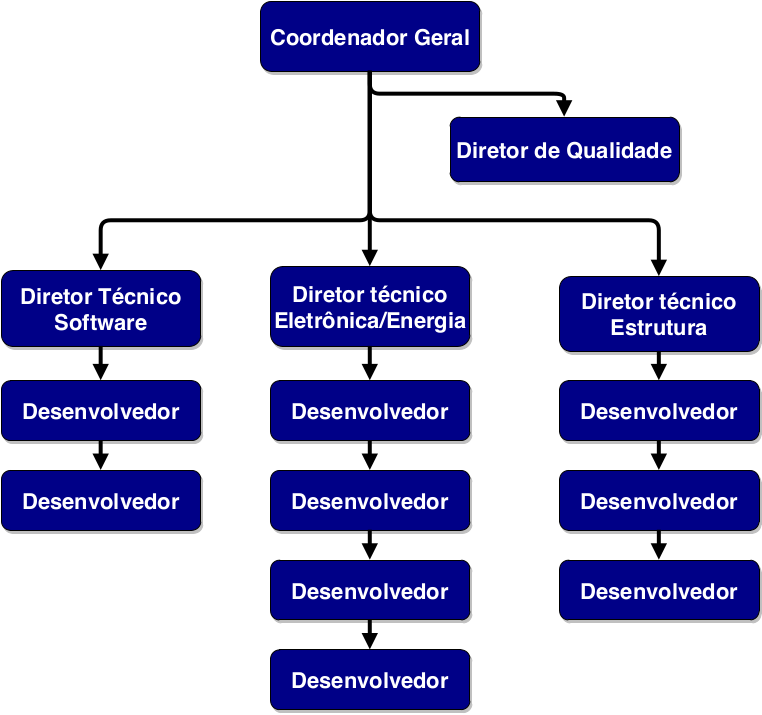
\includegraphics[scale = 0.5]{organograma}
\caption{.}\label{fig:organograma}
\end{figure} 

A seguir estão os nomes de cada integrante separado por área:

\begin{itemize}
\item Eletrônica e Energia

-Brenda Bianca Neves Dias\\
-Danyelle Bemfica da Rocha\\
-\textbf{Elpidio Cândido de Araújo Bisneto -> Coordenador geral}\\
-Filipe de Souza Freitas\\
-\textbf{Kewin Kuster -> Diretor técnico}\\
-Rodrigo Sousa Santos

\item Estrutura

-\textbf{Daniele Dias Sousa -> Diretora de qualidade}\\
-Fernanda Resende Muro Martinez\\
-Luiz Felipe Martins Cruz\\
-Pedro Henrique Nazareno Halabi\\
-\textbf{Rafael Mascarenhas dos Santos -> Diretor técnico}

\item Software

-Diego Barbosa da Mota França\\
-\textbf{João Pedro Sconetto -> Diretor técnico}\\
-Mariana de Souza Mendes 


\end{itemize}

\subsection{Ferramentas de gerenciamento}

Foram selecionadas algumas ferramentas de gerenciamento, afim de organizar o trabalho da equipe.

\emph{\textbf{Discord:}} É um aplicativo de comunicação onde a equipe pode se comunicar de forma rápida com mensagens, além disso permite o envio de vídeos, imagens e documentos. Outra vantagem da ferramenta é a possibilidade de fazer áudio-conferência com mais de 10 pessoas.

\emph{\textbf{Google drive:}} Ferramenta em nuvem para armazenamento e compartilhamento de arquivos.

\emph{\textbf{GitHub e Texmaker:}} \emph{Texmaker} é uma ferramenta para edição de texto em \emph{Latex} e o \emph{GitHub} é um ferramenta de desenvolvimento.

\emph{\textbf{Trello:}} O Trello é bastante conhecido por ser uma ferramenta de gerenciamento de projetos. 

\section{Cronograma de atividades}
\section{Milestones Identificados}
\section{Estimativa de custos}

\subsection{Engenharia de Software}

Aqui está listado todos os gastos que serão necessários para a equipe de software, assim como todas as aquisições que serão feitas durante o projeto:

\begin{table}[h]
    \resizebox{\textwidth}{!}{\begin{tabular}{@{}|c|c|c|c|c|c|c|@{}}
    \toprule
    \textbf{Nome do produto} & \textbf{Descrição}                      & \textbf{Marca} & \textbf{Preço unitário} & \textbf{Quantidade} & \textbf{Fornecedor} & \textbf{Orçamento} \\ \midrule
    Servidor                 & Máquina para execução dos serviços      & ---            & US\$ 10,00 por mês      & 5 meses             & Digital Ocean       & US\$ 50,00         \\ \midrule
    Raspberry Pi 3 B         & Placa de IoT para execução de softwares & Raspberry      & R\$ 279,90              & 1 unidade           & FilipeFlop          & R\$ 279,90         \\ \bottomrule
    \end{tabular}}
\end{table}

OBS: Essa planilha poderá ser atualizado dependendo de necessidades que surgirem durante a execução do projeto.


\subsection {Engenharia Eletrônica}

\subsubsection{Orçamento preliminar}
\begin{table}[h]
\centering
\caption{Estimativa de custos de eletrônica}
\label{custos_eletronica}
\begin{tabular}{|c|c|c|c|c|}
\hline
\multicolumn{5}{|c|}{Eletrônica} \\ \hline
Quantidade & Material & Valor Unitário & Total & Fornecedor \\ \hline
02 & BeagleBone & R\$ 320,00 & R\$ 640,00 & Mercado Livre \\ \hline
02 & Módulos GSM & R\$ 99,90 & R\$ 199,90 & TDTEC \\ \hline
02 & Módulos RF & R\$ 32,90 & R\$ 65,80 & HU Infinito \\ \hline
10 & \begin{tabular}[c]{@{}c@{}}Componentes para Placa\\  de Circuito Impresso\end{tabular} & R\$ 40,00 & R\$ 400,00 & HU Infinito \\ \hline
02 & Antena painel & R\$ 108,80 & R\$ 217,60 & Emprestado \\ \hline
02 & BladeRF NUAND & R\$ 3.000,00 & R\$ 6.000,00 & Emprestado \\ \hline
02 & Circulador & R\$ 150,00 & R\$ 300,00 & Emprestado \\ \hline
02 & Câmera & R\$ 1.000,00 & R\$ 2.000,00 & Em análise \\ \hline
X & Componentes diversos & R\$ 50,00 & R\$ 50,00 & HU Infinito \\ \hline
Total & - - & - - & R\$ 9873,30 & - - \\ \hline
\end{tabular}
\end{table}


\section{Viabilidades financeira}
\section{Levantamento de riscos}
\subsection{Geral}

\begin{itemize}
    \item RGN 1 - Saída de um membro da equipe;
    \item RGN 2 - Desentendimentos entre membros da equipe;
    \item RGN 3 - Membro da equipe temporariamente impossibilitado de trabalhar;
    \item RGN 4 - Mudança do escopo do projeto;
    \item RGN 5 - Equipe com dificuldades no uso das tecnologias usadas no projeto;
    \item RGN 6 - Dívida técnica por não conseguir entregar as histórias previstas;
    \item RGN 7 - Membros com carga excessiva de trabalho;
    \item RGN 8 - Atraso no roadmap do projeto.
\end{itemize}

\subsection{Software}
\begin{itemize}
    \item RSN 1 - Falta de infraestrutura para o desenvolvimento do software (configuração de ambiente de desenvolvimento, configuração do github, etc);
    \item RSN 2 - Descontinuação de pacotes de dependências usados;
    \item RSN 3 - Dificuldades para realizar o deploy;
    \item RSN 4 - Atraso na implementação da arquitetura do projeto;
    \item RSN 5 - Dificuldades com as tecnologias relacionadas à microsserviços;
    \item RSN 6 - Problemas na comunicação entre os softwares e o radar.
\end{itemize}

\subsubsection{Energia}
\begin{itemize}
   \item Alimentação insuficiente ao Radar;
   \item Curta vida útil dos equipamentos; 
   \item Queima dos componentes elétricos;
   \item Tamanho da bitola dos cabos insuficiente para a quantidade de tensão e corrente;
   \item Montagem mal feita;
   \item Altura da fonte de alimentação segura para realizar manutenção e instalação;
   \item Pista movimentada no dia da instalação;
   \item Negligenciamento da dissipação de calor;
   \item Estrutura mal dimensionada para o suporte e proteção do sistema de alimentação
\end{itemize}
